\documentclass{standalone}
\usepackage{tikz}
\usetikzlibrary{patterns, positioning}


\begin{document}
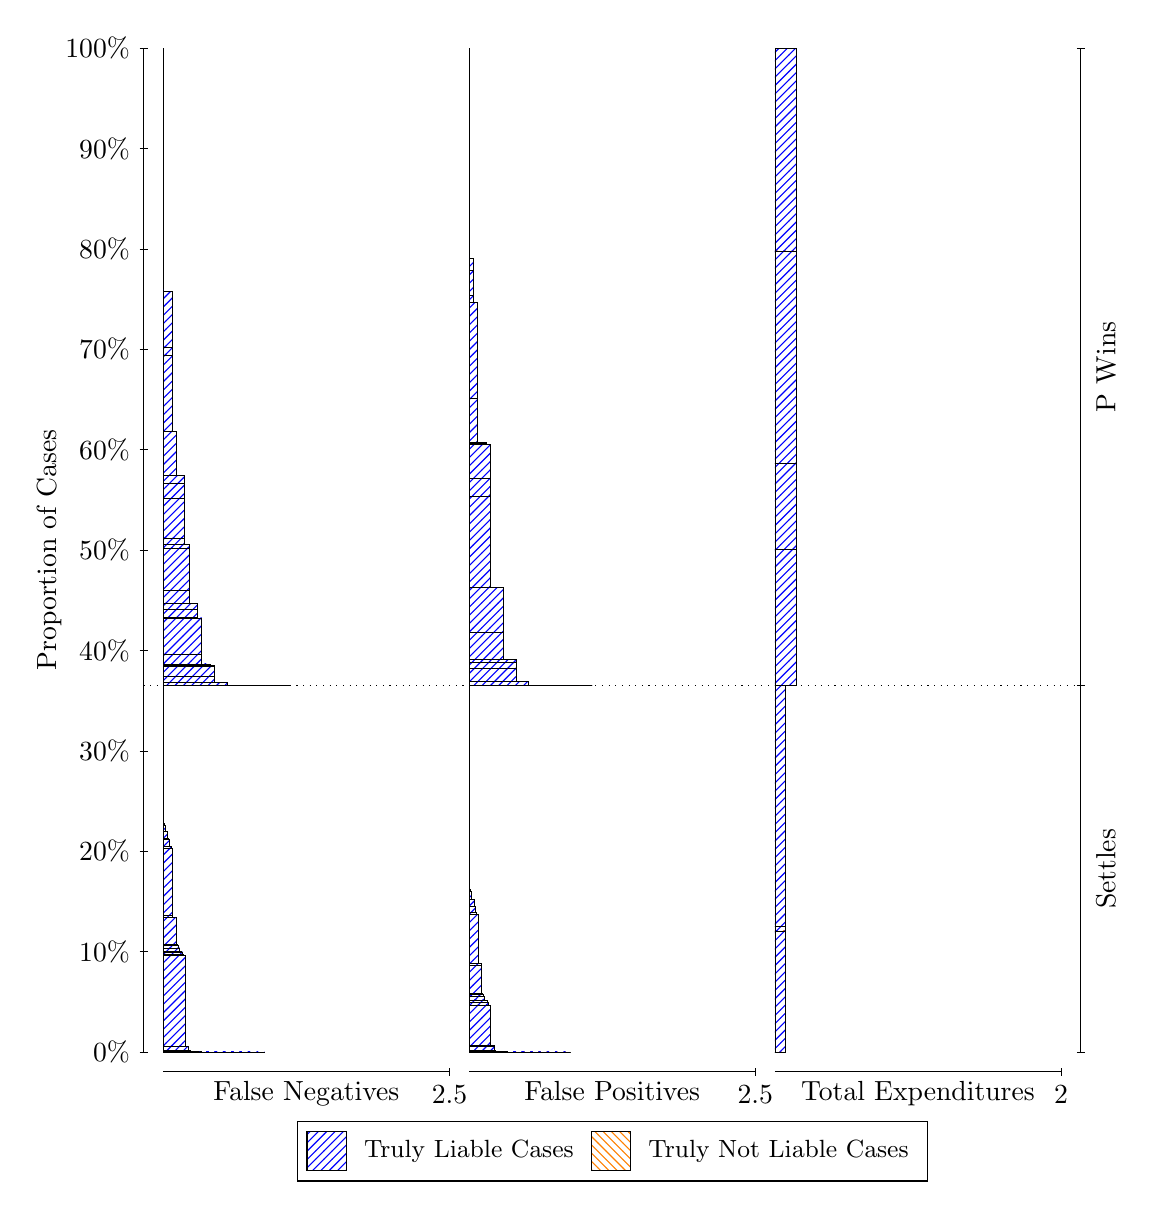
\begin{tikzpicture}
\draw[black, very thin] (1.5,1.75) -- (1.5,14.5);
\node[rotate=90, text=black, anchor=center] at (0.3, 8.125) {Proportion of Cases};
\draw[black, very thin] (1.45,1.75) -- (1.55,1.75);
\node[text=black, anchor=east] at (1.45, 1.75) {0\%};
\draw[black, very thin] (1.45,3.025) -- (1.55,3.025);
\node[text=black, anchor=east] at (1.45, 3.025) {10\%};
\draw[black, very thin] (1.45,4.3) -- (1.55,4.3);
\node[text=black, anchor=east] at (1.45, 4.3) {20\%};
\draw[black, very thin] (1.45,5.575) -- (1.55,5.575);
\node[text=black, anchor=east] at (1.45, 5.575) {30\%};
\draw[black, very thin] (1.45,6.85) -- (1.55,6.85);
\node[text=black, anchor=east] at (1.45, 6.85) {40\%};
\draw[black, very thin] (1.45,8.125) -- (1.55,8.125);
\node[text=black, anchor=east] at (1.45, 8.125) {50\%};
\draw[black, very thin] (1.45,9.4) -- (1.55,9.4);
\node[text=black, anchor=east] at (1.45, 9.4) {60\%};
\draw[black, very thin] (1.45,10.675) -- (1.55,10.675);
\node[text=black, anchor=east] at (1.45, 10.675) {70\%};
\draw[black, very thin] (1.45,11.95) -- (1.55,11.95);
\node[text=black, anchor=east] at (1.45, 11.95) {80\%};
\draw[black, very thin] (1.45,13.225) -- (1.55,13.225);
\node[text=black, anchor=east] at (1.45, 13.225) {90\%};
\draw[black, very thin] (1.45,14.5) -- (1.55,14.5);
\node[text=black, anchor=east] at (1.45, 14.5) {100\%};

\draw[black, very thin] (13.4,1.75) -- (13.4,14.5);
\draw[black, very thin] (13.35,1.75) -- (13.45,1.75);
\node[anchor=west] at (13.35, 1.75) {};
\draw[black, very thin] (13.35,6.4014) -- (13.45,6.4014);
\node[anchor=west] at (13.35, 6.4014) {};
\draw[black, very thin] (13.35,14.5) -- (13.45,14.5);
\node[anchor=west] at (13.35, 14.5) {};

\draw[black, very thin, pattern color=blue, pattern=north east lines] (1.75,1.75) rectangle (3.0398,1.75);
\draw[black, very thin, pattern color=blue, pattern=north east lines] (1.75,1.75) rectangle (2.8945,1.75);
\draw[black, very thin, pattern color=blue, pattern=north east lines] (1.75,1.75) rectangle (2.8784,1.75);
\draw[black, very thin, pattern color=blue, pattern=north east lines] (1.75,1.75) rectangle (2.8218,1.75);
\draw[black, very thin, pattern color=blue, pattern=north east lines] (1.75,1.75) rectangle (2.7492,1.75);
\draw[black, very thin, pattern color=blue, pattern=north east lines] (1.75,1.75) rectangle (2.733,1.75);
\draw[black, very thin, pattern color=blue, pattern=north east lines] (1.75,1.75) rectangle (2.7169,1.75);
\draw[black, very thin, pattern color=blue, pattern=north east lines] (1.75,1.75) rectangle (2.6765,1.75);
\draw[black, very thin, pattern color=blue, pattern=north east lines] (1.75,1.75) rectangle (2.6604,1.75);
\draw[black, very thin, pattern color=blue, pattern=north east lines] (1.75,1.75) rectangle (2.6038,1.75);
\draw[black, very thin, pattern color=blue, pattern=north east lines] (1.75,1.75) rectangle (2.5877,1.75);
\draw[black, very thin, pattern color=blue, pattern=north east lines] (1.75,1.75) rectangle (2.5715,1.75);
\draw[black, very thin, pattern color=blue, pattern=north east lines] (1.75,1.75) rectangle (2.5554,1.75);
\draw[black, very thin, pattern color=blue, pattern=north east lines] (1.75,1.75) rectangle (2.5312,1.75);
\draw[black, very thin, pattern color=blue, pattern=north east lines] (1.75,1.75) rectangle (2.515,1.75);
\draw[black, very thin, pattern color=blue, pattern=north east lines] (1.75,1.75) rectangle (2.4989,1.75);
\draw[black, very thin, pattern color=blue, pattern=north east lines] (1.75,1.75) rectangle (2.4585,1.75);
\draw[black, very thin, pattern color=blue, pattern=north east lines] (1.75,1.75) rectangle (2.4424,1.75);
\draw[black, very thin, pattern color=blue, pattern=north east lines] (1.75,1.75) rectangle (2.4262,1.75);
\draw[black, very thin, pattern color=blue, pattern=north east lines] (1.75,1.75) rectangle (2.4101,1.75);
\draw[black, very thin, pattern color=blue, pattern=north east lines] (1.75,1.75) rectangle (2.3939,1.75);
\draw[black, very thin, pattern color=blue, pattern=north east lines] (1.75,1.75) rectangle (2.3858,1.75);
\draw[black, very thin, pattern color=blue, pattern=north east lines] (1.75,1.75) rectangle (2.3697,1.75);
\draw[black, very thin, pattern color=blue, pattern=north east lines] (1.75,1.75) rectangle (2.3535,1.75);
\draw[black, very thin, pattern color=blue, pattern=north east lines] (1.75,1.75) rectangle (2.3374,1.75);
\draw[black, very thin, pattern color=blue, pattern=north east lines] (1.75,1.75) rectangle (2.3132,1.7501);
\draw[black, very thin, pattern color=blue, pattern=north east lines] (1.75,1.7501) rectangle (2.297,1.7501);
\draw[black, very thin, pattern color=blue, pattern=north east lines] (1.75,1.7501) rectangle (2.2809,1.7502);
\draw[black, very thin, pattern color=blue, pattern=north east lines] (1.75,1.7502) rectangle (2.2647,1.7502);
\draw[black, very thin, pattern color=blue, pattern=north east lines] (1.75,1.7502) rectangle (2.2486,1.7502);
\draw[black, very thin, pattern color=blue, pattern=north east lines] (1.75,1.7502) rectangle (2.2324,1.7527);
\draw[black, very thin, pattern color=blue, pattern=north east lines] (1.75,1.7527) rectangle (2.2244,1.7527);
\draw[black, very thin, pattern color=blue, pattern=north east lines] (1.75,1.7527) rectangle (2.2082,1.7527);
\draw[black, very thin, pattern color=blue, pattern=north east lines] (1.75,1.7527) rectangle (2.1921,1.7529);
\draw[black, very thin, pattern color=blue, pattern=north east lines] (1.75,1.7529) rectangle (2.1759,1.7531);
\draw[black, very thin, pattern color=blue, pattern=north east lines] (1.75,1.7531) rectangle (2.1678,1.7534);
\draw[black, very thin, pattern color=blue, pattern=north east lines] (1.75,1.7534) rectangle (2.1517,1.7556);
\draw[black, very thin, pattern color=blue, pattern=north east lines] (1.75,1.7556) rectangle (2.1355,1.7558);
\draw[black, very thin, pattern color=blue, pattern=north east lines] (1.75,1.7558) rectangle (2.1194,1.7605);
\draw[black, very thin, pattern color=blue, pattern=north east lines] (1.75,1.7605) rectangle (2.1032,1.7624);
\draw[black, very thin, pattern color=blue, pattern=north east lines] (1.75,1.7624) rectangle (2.0871,1.7654);
\draw[black, very thin, pattern color=blue, pattern=north east lines] (1.75,1.7654) rectangle (2.0709,1.8236);
\draw[black, very thin, pattern color=blue, pattern=north east lines] (1.75,1.8236) rectangle (2.0629,1.8236);
\draw[black, very thin, pattern color=blue, pattern=north east lines] (1.75,1.8236) rectangle (2.0467,1.8237);
\draw[black, very thin, pattern color=blue, pattern=north east lines] (1.75,1.8237) rectangle (2.0306,1.8284);
\draw[black, very thin, pattern color=blue, pattern=north east lines] (1.75,1.8284) rectangle (2.0225,2.9799);
\draw[black, very thin, pattern color=blue, pattern=north east lines] (1.75,2.9799) rectangle (2.0144,2.9823);
\draw[black, very thin, pattern color=blue, pattern=north east lines] (1.75,2.9823) rectangle (2.0064,2.9879);
\draw[black, very thin, pattern color=blue, pattern=north east lines] (1.75,2.9879) rectangle (1.9902,3.0209);
\draw[black, very thin, pattern color=blue, pattern=north east lines] (1.75,3.0209) rectangle (1.9741,3.0228);
\draw[black, very thin, pattern color=blue, pattern=north east lines] (1.75,3.0228) rectangle (1.9579,3.071);
\draw[black, very thin, pattern color=blue, pattern=north east lines] (1.75,3.071) rectangle (1.9418,3.1006);
\draw[black, very thin, pattern color=blue, pattern=north east lines] (1.75,3.1006) rectangle (1.9256,3.1212);
\draw[black, very thin, pattern color=blue, pattern=north east lines] (1.75,3.1212) rectangle (1.9095,3.4593);
\draw[black, very thin, pattern color=blue, pattern=north east lines] (1.75,3.4593) rectangle (1.9014,3.4593);
\draw[black, very thin, pattern color=blue, pattern=north east lines] (1.75,3.4593) rectangle (1.8852,3.4598);
\draw[black, very thin, pattern color=blue, pattern=north east lines] (1.75,3.4598) rectangle (1.8691,3.4832);
\draw[black, very thin, pattern color=blue, pattern=north east lines] (1.75,3.4832) rectangle (1.861,4.331);
\draw[black, very thin, pattern color=blue, pattern=north east lines] (1.75,4.331) rectangle (1.8529,4.3367);
\draw[black, very thin, pattern color=blue, pattern=north east lines] (1.75,4.3367) rectangle (1.8449,4.3626);
\draw[black, very thin, pattern color=blue, pattern=north east lines] (1.75,4.3626) rectangle (1.8287,4.4564);
\draw[black, very thin, pattern color=blue, pattern=north east lines] (1.75,4.4564) rectangle (1.8126,4.461);
\draw[black, very thin, pattern color=blue, pattern=north east lines] (1.75,4.461) rectangle (1.7964,4.5542);
\draw[black, very thin, pattern color=blue, pattern=north east lines] (1.75,4.5542) rectangle (1.7803,4.6288);
\draw[black, very thin, pattern color=blue, pattern=north east lines] (1.75,4.6288) rectangle (1.7641,4.6524);
\draw[black, very thin, pattern color=orange, pattern=north west lines] (1.75,4.6524) rectangle (1.75,4.6524);
\draw[black, very thin, pattern color=blue, pattern=north east lines] (1.75,4.6524) rectangle (1.75,6.4014);
\draw[black, very thin, pattern color=blue, pattern=north east lines] (1.75,6.4014) rectangle (3.3668,6.4014);
\draw[black, very thin, pattern color=blue, pattern=north east lines] (1.75,6.4014) rectangle (3.2054,6.4014);
\draw[black, very thin, pattern color=blue, pattern=north east lines] (1.75,6.4014) rectangle (3.1509,6.4014);
\draw[black, very thin, pattern color=blue, pattern=north east lines] (1.75,6.4014) rectangle (3.0439,6.4014);
\draw[black, very thin, pattern color=blue, pattern=north east lines] (1.75,6.4014) rectangle (2.9894,6.4014);
\draw[black, very thin, pattern color=blue, pattern=north east lines] (1.75,6.4014) rectangle (2.9894,6.4014);
\draw[black, very thin, pattern color=blue, pattern=north east lines] (1.75,6.4014) rectangle (2.8824,6.4016);
\draw[black, very thin, pattern color=blue, pattern=north east lines] (1.75,6.4016) rectangle (2.8824,6.4018);
\draw[black, very thin, pattern color=blue, pattern=north east lines] (1.75,6.4018) rectangle (2.8279,6.4018);
\draw[black, very thin, pattern color=blue, pattern=north east lines] (1.75,6.4018) rectangle (2.7209,6.4045);
\draw[black, very thin, pattern color=blue, pattern=north east lines] (1.75,6.4045) rectangle (2.7209,6.4065);
\draw[black, very thin, pattern color=blue, pattern=north east lines] (1.75,6.4065) rectangle (2.6664,6.4065);
\draw[black, very thin, pattern color=blue, pattern=north east lines] (1.75,6.4065) rectangle (2.5594,6.4483);
\draw[black, very thin, pattern color=blue, pattern=north east lines] (1.75,6.4483) rectangle (2.5049,6.4483);
\draw[black, very thin, pattern color=blue, pattern=north east lines] (1.75,6.4483) rectangle (2.5049,6.4485);
\draw[black, very thin, pattern color=blue, pattern=north east lines] (1.75,6.4485) rectangle (2.3979,6.5231);
\draw[black, very thin, pattern color=blue, pattern=north east lines] (1.75,6.5231) rectangle (2.3979,6.6477);
\draw[black, very thin, pattern color=blue, pattern=north east lines] (1.75,6.6477) rectangle (2.3979,6.6625);
\draw[black, very thin, pattern color=blue, pattern=north east lines] (1.75,6.6625) rectangle (2.3434,6.6661);
\draw[black, very thin, pattern color=blue, pattern=north east lines] (1.75,6.6661) rectangle (2.3434,6.6738);
\draw[black, very thin, pattern color=blue, pattern=north east lines] (1.75,6.6738) rectangle (2.3434,6.6779);
\draw[black, very thin, pattern color=blue, pattern=north east lines] (1.75,6.6779) rectangle (2.2365,6.7971);
\draw[black, very thin, pattern color=blue, pattern=north east lines] (1.75,6.7971) rectangle (2.2365,7.2633);
\draw[black, very thin, pattern color=blue, pattern=north east lines] (1.75,7.2633) rectangle (2.182,7.2727);
\draw[black, very thin, pattern color=blue, pattern=north east lines] (1.75,7.2727) rectangle (2.182,7.3726);
\draw[black, very thin, pattern color=blue, pattern=north east lines] (1.75,7.3726) rectangle (2.182,7.4495);
\draw[black, very thin, pattern color=blue, pattern=north east lines] (1.75,7.4495) rectangle (2.075,7.6114);
\draw[black, very thin, pattern color=blue, pattern=north east lines] (1.75,7.6114) rectangle (2.075,8.1521);
\draw[black, very thin, pattern color=blue, pattern=north east lines] (1.75,8.1521) rectangle (2.075,8.1974);
\draw[black, very thin, pattern color=blue, pattern=north east lines] (1.75,8.1974) rectangle (2.0205,8.2801);
\draw[black, very thin, pattern color=blue, pattern=north east lines] (1.75,8.2801) rectangle (2.0205,8.7853);
\draw[black, very thin, pattern color=blue, pattern=north east lines] (1.75,8.7853) rectangle (2.0205,8.9719);
\draw[black, very thin, pattern color=blue, pattern=north east lines] (1.75,8.9719) rectangle (2.0205,9.077);
\draw[black, very thin, pattern color=blue, pattern=north east lines] (1.75,9.077) rectangle (1.9135,9.6344);
\draw[black, very thin, pattern color=blue, pattern=north east lines] (1.75,9.6344) rectangle (1.859,10.603);
\draw[black, very thin, pattern color=blue, pattern=north east lines] (1.75,10.603) rectangle (1.859,10.705);
\draw[black, very thin, pattern color=blue, pattern=north east lines] (1.75,10.705) rectangle (1.859,11.408);
\draw[black, very thin, pattern color=blue, pattern=north east lines] (1.75,11.408) rectangle (1.752,11.438);
\draw[black, very thin, pattern color=blue, pattern=north east lines] (1.75,11.438) rectangle (1.752,11.438);
\draw[black, very thin, pattern color=orange, pattern=north west lines] (1.75,11.438) rectangle (1.75,11.438);
\draw[black, very thin, pattern color=blue, pattern=north east lines] (1.75,11.438) rectangle (1.75,14.5);
\draw[black, very thin, pattern color=orange, pattern=north west lines] (5.6333,1.75) rectangle (6.9232,1.75);
\draw[black, very thin, pattern color=blue, pattern=north east lines] (5.6333,1.75) rectangle (6.9232,1.75);
\draw[black, very thin, pattern color=orange, pattern=north west lines] (5.6333,1.75) rectangle (6.7778,1.75);
\draw[black, very thin, pattern color=blue, pattern=north east lines] (5.6333,1.75) rectangle (6.7778,1.75);
\draw[black, very thin, pattern color=blue, pattern=north east lines] (5.6333,1.75) rectangle (6.7617,1.75);
\draw[black, very thin, pattern color=orange, pattern=north west lines] (5.6333,1.75) rectangle (6.6325,1.75);
\draw[black, very thin, pattern color=blue, pattern=north east lines] (5.6333,1.75) rectangle (6.6325,1.75);
\draw[black, very thin, pattern color=blue, pattern=north east lines] (5.6333,1.75) rectangle (6.6164,1.75);
\draw[black, very thin, pattern color=blue, pattern=north east lines] (5.6333,1.75) rectangle (6.6002,1.75);
\draw[black, very thin, pattern color=orange, pattern=north west lines] (5.6333,1.75) rectangle (6.5598,1.75);
\draw[black, very thin, pattern color=blue, pattern=north east lines] (5.6333,1.75) rectangle (6.5598,1.75);
\draw[black, very thin, pattern color=orange, pattern=north west lines] (5.6333,1.75) rectangle (6.4872,1.75);
\draw[black, very thin, pattern color=blue, pattern=north east lines] (5.6333,1.75) rectangle (6.4872,1.75);
\draw[black, very thin, pattern color=blue, pattern=north east lines] (5.6333,1.75) rectangle (6.471,1.75);
\draw[black, very thin, pattern color=blue, pattern=north east lines] (5.6333,1.75) rectangle (6.4549,1.75);
\draw[black, very thin, pattern color=blue, pattern=north east lines] (5.6333,1.75) rectangle (6.4387,1.75);
\draw[black, very thin, pattern color=orange, pattern=north west lines] (5.6333,1.75) rectangle (6.4145,1.75);
\draw[black, very thin, pattern color=blue, pattern=north east lines] (5.6333,1.75) rectangle (6.4145,1.75);
\draw[black, very thin, pattern color=blue, pattern=north east lines] (5.6333,1.75) rectangle (6.3984,1.75);
\draw[black, very thin, pattern color=orange, pattern=north west lines] (5.6333,1.75) rectangle (6.3418,1.75);
\draw[black, very thin, pattern color=blue, pattern=north east lines] (5.6333,1.75) rectangle (6.3418,1.75);
\draw[black, very thin, pattern color=blue, pattern=north east lines] (5.6333,1.75) rectangle (6.3257,1.75);
\draw[black, very thin, pattern color=blue, pattern=north east lines] (5.6333,1.75) rectangle (6.3095,1.75);
\draw[black, very thin, pattern color=blue, pattern=north east lines] (5.6333,1.75) rectangle (6.2934,1.75);
\draw[black, very thin, pattern color=blue, pattern=north east lines] (5.6333,1.75) rectangle (6.2772,1.75);
\draw[black, very thin, pattern color=orange, pattern=north west lines] (5.6333,1.75) rectangle (6.2692,1.75);
\draw[black, very thin, pattern color=blue, pattern=north east lines] (5.6333,1.75) rectangle (6.2692,1.75);
\draw[black, very thin, pattern color=blue, pattern=north east lines] (5.6333,1.75) rectangle (6.253,1.75);
\draw[black, very thin, pattern color=blue, pattern=north east lines] (5.6333,1.75) rectangle (6.2369,1.75);
\draw[black, very thin, pattern color=orange, pattern=north west lines] (5.6333,1.75) rectangle (6.1965,1.75);
\draw[black, very thin, pattern color=blue, pattern=north east lines] (5.6333,1.75) rectangle (6.1965,1.7501);
\draw[black, very thin, pattern color=blue, pattern=north east lines] (5.6333,1.7501) rectangle (6.1804,1.7501);
\draw[black, very thin, pattern color=blue, pattern=north east lines] (5.6333,1.7501) rectangle (6.1642,1.7501);
\draw[black, very thin, pattern color=blue, pattern=north east lines] (5.6333,1.7501) rectangle (6.1481,1.7502);
\draw[black, very thin, pattern color=blue, pattern=north east lines] (5.6333,1.7502) rectangle (6.1319,1.7504);
\draw[black, very thin, pattern color=orange, pattern=north west lines] (5.6333,1.7504) rectangle (6.1238,1.7504);
\draw[black, very thin, pattern color=blue, pattern=north east lines] (5.6333,1.7504) rectangle (6.1238,1.7504);
\draw[black, very thin, pattern color=blue, pattern=north east lines] (5.6333,1.7504) rectangle (6.1158,1.7528);
\draw[black, very thin, pattern color=blue, pattern=north east lines] (5.6333,1.7528) rectangle (6.1077,1.7529);
\draw[black, very thin, pattern color=blue, pattern=north east lines] (5.6333,1.7529) rectangle (6.0915,1.7529);
\draw[black, very thin, pattern color=blue, pattern=north east lines] (5.6333,1.7529) rectangle (6.0754,1.7529);
\draw[black, very thin, pattern color=orange, pattern=north west lines] (5.6333,1.7529) rectangle (6.0512,1.7529);
\draw[black, very thin, pattern color=blue, pattern=north east lines] (5.6333,1.7529) rectangle (6.0512,1.7533);
\draw[black, very thin, pattern color=blue, pattern=north east lines] (5.6333,1.7533) rectangle (6.035,1.7554);
\draw[black, very thin, pattern color=blue, pattern=north east lines] (5.6333,1.7554) rectangle (6.0189,1.7573);
\draw[black, very thin, pattern color=blue, pattern=north east lines] (5.6333,1.7573) rectangle (6.0027,1.7574);
\draw[black, very thin, pattern color=blue, pattern=north east lines] (5.6333,1.7574) rectangle (5.9866,1.7623);
\draw[black, very thin, pattern color=blue, pattern=north east lines] (5.6333,1.7623) rectangle (5.9704,1.7672);
\draw[black, very thin, pattern color=blue, pattern=north east lines] (5.6333,1.7672) rectangle (5.9624,1.7674);
\draw[black, very thin, pattern color=blue, pattern=north east lines] (5.6333,1.7674) rectangle (5.9543,1.8261);
\draw[black, very thin, pattern color=blue, pattern=north east lines] (5.6333,1.8261) rectangle (5.9462,1.8292);
\draw[black, very thin, pattern color=blue, pattern=north east lines] (5.6333,1.8292) rectangle (5.9301,1.8293);
\draw[black, very thin, pattern color=blue, pattern=north east lines] (5.6333,1.8293) rectangle (5.9139,1.8293);
\draw[black, very thin, pattern color=orange, pattern=north west lines] (5.6333,1.8293) rectangle (5.9058,1.8293);
\draw[black, very thin, pattern color=blue, pattern=north east lines] (5.6333,1.8293) rectangle (5.9058,2.3428);
\draw[black, very thin, pattern color=blue, pattern=north east lines] (5.6333,2.3428) rectangle (5.8897,2.3483);
\draw[black, very thin, pattern color=blue, pattern=north east lines] (5.6333,2.3483) rectangle (5.8735,2.3783);
\draw[black, very thin, pattern color=blue, pattern=north east lines] (5.6333,2.3783) rectangle (5.8574,2.4108);
\draw[black, very thin, pattern color=blue, pattern=north east lines] (5.6333,2.4108) rectangle (5.8412,2.4126);
\draw[black, very thin, pattern color=blue, pattern=north east lines] (5.6333,2.4126) rectangle (5.8251,2.4614);
\draw[black, very thin, pattern color=blue, pattern=north east lines] (5.6333,2.4614) rectangle (5.8089,2.487);
\draw[black, very thin, pattern color=blue, pattern=north east lines] (5.6333,2.487) rectangle (5.8009,2.4895);
\draw[black, very thin, pattern color=blue, pattern=north east lines] (5.6333,2.4895) rectangle (5.7928,2.8513);
\draw[black, very thin, pattern color=blue, pattern=north east lines] (5.6333,2.8513) rectangle (5.7847,2.8718);
\draw[black, very thin, pattern color=blue, pattern=north east lines] (5.6333,2.8718) rectangle (5.7686,2.8723);
\draw[black, very thin, pattern color=blue, pattern=north east lines] (5.6333,2.8723) rectangle (5.7524,2.8723);
\draw[black, very thin, pattern color=blue, pattern=north east lines] (5.6333,2.8723) rectangle (5.7444,3.499);
\draw[black, very thin, pattern color=blue, pattern=north east lines] (5.6333,3.499) rectangle (5.7282,3.5227);
\draw[black, very thin, pattern color=blue, pattern=north east lines] (5.6333,3.5227) rectangle (5.7121,3.5972);
\draw[black, very thin, pattern color=blue, pattern=north east lines] (5.6333,3.5972) rectangle (5.6959,3.6904);
\draw[black, very thin, pattern color=blue, pattern=north east lines] (5.6333,3.6904) rectangle (5.6798,3.6951);
\draw[black, very thin, pattern color=blue, pattern=north east lines] (5.6333,3.6951) rectangle (5.6636,3.7888);
\draw[black, very thin, pattern color=blue, pattern=north east lines] (5.6333,3.7888) rectangle (5.6475,3.8148);
\draw[black, very thin, pattern color=blue, pattern=north east lines] (5.6333,3.8148) rectangle (5.6394,3.8204);
\draw[black, very thin, pattern color=blue, pattern=north east lines] (5.6333,3.8204) rectangle (5.6333,6.4014);
\draw[black, very thin, pattern color=orange, pattern=north west lines] (5.6333,6.4014) rectangle (7.1957,6.4014);
\draw[black, very thin, pattern color=blue, pattern=north east lines] (5.6333,6.4014) rectangle (7.1957,6.4014);
\draw[black, very thin, pattern color=orange, pattern=north west lines] (5.6333,6.4014) rectangle (7.0342,6.4014);
\draw[black, very thin, pattern color=blue, pattern=north east lines] (5.6333,6.4014) rectangle (7.0342,6.4014);
\draw[black, very thin, pattern color=orange, pattern=north west lines] (5.6333,6.4014) rectangle (6.8727,6.4014);
\draw[black, very thin, pattern color=blue, pattern=north east lines] (5.6333,6.4014) rectangle (6.8727,6.4015);
\draw[black, very thin, pattern color=blue, pattern=north east lines] (5.6333,6.4015) rectangle (6.8727,6.4015);
\draw[black, very thin, pattern color=blue, pattern=north east lines] (5.6333,6.4015) rectangle (6.7112,6.4017);
\draw[black, very thin, pattern color=orange, pattern=north west lines] (5.6333,6.4017) rectangle (6.7112,6.4017);
\draw[black, very thin, pattern color=blue, pattern=north east lines] (5.6333,6.4017) rectangle (6.7112,6.4019);
\draw[black, very thin, pattern color=orange, pattern=north west lines] (5.6333,6.4019) rectangle (6.5497,6.4019);
\draw[black, very thin, pattern color=blue, pattern=north east lines] (5.6333,6.4019) rectangle (6.5497,6.4081);
\draw[black, very thin, pattern color=orange, pattern=north west lines] (5.6333,6.4081) rectangle (6.4952,6.4081);
\draw[black, very thin, pattern color=blue, pattern=north east lines] (5.6333,6.4081) rectangle (6.4952,6.4081);
\draw[black, very thin, pattern color=orange, pattern=north west lines] (5.6333,6.4081) rectangle (6.3883,6.4081);
\draw[black, very thin, pattern color=blue, pattern=north east lines] (5.6333,6.4081) rectangle (6.3883,6.4609);
\draw[black, very thin, pattern color=blue, pattern=north east lines] (5.6333,6.4609) rectangle (6.3338,6.4609);
\draw[black, very thin, pattern color=orange, pattern=north west lines] (5.6333,6.4609) rectangle (6.3338,6.4609);
\draw[black, very thin, pattern color=blue, pattern=north east lines] (5.6333,6.4609) rectangle (6.3338,6.4609);
\draw[black, very thin, pattern color=orange, pattern=north west lines] (5.6333,6.4609) rectangle (6.2268,6.4609);
\draw[black, very thin, pattern color=blue, pattern=north east lines] (5.6333,6.4609) rectangle (6.2268,6.6259);
\draw[black, very thin, pattern color=blue, pattern=north east lines] (5.6333,6.6259) rectangle (6.2268,6.6955);
\draw[black, very thin, pattern color=blue, pattern=north east lines] (5.6333,6.6955) rectangle (6.2268,6.7396);
\draw[black, very thin, pattern color=blue, pattern=north east lines] (5.6333,6.7396) rectangle (6.1723,6.7396);
\draw[black, very thin, pattern color=orange, pattern=north west lines] (5.6333,6.7396) rectangle (6.1723,6.7396);
\draw[black, very thin, pattern color=blue, pattern=north east lines] (5.6333,6.7396) rectangle (6.1723,6.7396);
\draw[black, very thin, pattern color=orange, pattern=north west lines] (5.6333,6.7396) rectangle (6.0653,6.7396);
\draw[black, very thin, pattern color=blue, pattern=north east lines] (5.6333,6.7396) rectangle (6.0653,7.0767);
\draw[black, very thin, pattern color=blue, pattern=north east lines] (5.6333,7.0767) rectangle (6.0653,7.6523);
\draw[black, very thin, pattern color=blue, pattern=north east lines] (5.6333,7.6523) rectangle (6.0108,7.6523);
\draw[black, very thin, pattern color=orange, pattern=north west lines] (5.6333,7.6523) rectangle (6.0108,7.6523);
\draw[black, very thin, pattern color=blue, pattern=north east lines] (5.6333,7.6523) rectangle (6.0108,7.6525);
\draw[black, very thin, pattern color=orange, pattern=north west lines] (5.6333,7.6525) rectangle (5.9038,7.6525);
\draw[black, very thin, pattern color=blue, pattern=north east lines] (5.6333,7.6525) rectangle (5.9038,8.8093);
\draw[black, very thin, pattern color=blue, pattern=north east lines] (5.6333,8.8093) rectangle (5.9038,9.0299);
\draw[black, very thin, pattern color=blue, pattern=north east lines] (5.6333,9.0299) rectangle (5.9038,9.4635);
\draw[black, very thin, pattern color=blue, pattern=north east lines] (5.6333,9.4635) rectangle (5.8493,9.4636);
\draw[black, very thin, pattern color=orange, pattern=north west lines] (5.6333,9.4636) rectangle (5.8493,9.4636);
\draw[black, very thin, pattern color=blue, pattern=north east lines] (5.6333,9.4636) rectangle (5.8493,9.482);
\draw[black, very thin, pattern color=blue, pattern=north east lines] (5.6333,9.482) rectangle (5.8493,9.4932);
\draw[black, very thin, pattern color=blue, pattern=north east lines] (5.6333,9.4932) rectangle (5.7423,10.046);
\draw[black, very thin, pattern color=blue, pattern=north east lines] (5.6333,10.046) rectangle (5.7423,11.267);
\draw[black, very thin, pattern color=blue, pattern=north east lines] (5.6333,11.267) rectangle (5.6878,11.363);
\draw[black, very thin, pattern color=orange, pattern=north west lines] (5.6333,11.363) rectangle (5.6878,11.363);
\draw[black, very thin, pattern color=blue, pattern=north east lines] (5.6333,11.363) rectangle (5.6878,11.678);
\draw[black, very thin, pattern color=blue, pattern=north east lines] (5.6333,11.678) rectangle (5.6878,11.824);
\draw[black, very thin, pattern color=blue, pattern=north east lines] (5.6333,11.824) rectangle (5.6333,14.5);
\draw[black, very thin, pattern color=orange, pattern=north west lines] (9.5167,1.75) rectangle (9.6529,1.75);
\draw[black, very thin, pattern color=blue, pattern=north east lines] (9.5167,1.75) rectangle (9.6529,3.2891);
\draw[black, very thin, pattern color=orange, pattern=north west lines] (9.5167,3.2891) rectangle (9.6529,3.2891);
\draw[black, very thin, pattern color=blue, pattern=north east lines] (9.5167,3.2891) rectangle (9.6529,3.3422);
\draw[black, very thin, pattern color=orange, pattern=north west lines] (9.5167,3.3422) rectangle (9.6529,3.3422);
\draw[black, very thin, pattern color=blue, pattern=north east lines] (9.5167,3.3422) rectangle (9.6529,6.4014);
\draw[black, very thin, pattern color=orange, pattern=north west lines] (9.5167,6.4014) rectangle (9.7892,6.4014);
\draw[black, very thin, pattern color=blue, pattern=north east lines] (9.5167,6.4014) rectangle (9.7892,8.1355);
\draw[black, very thin, pattern color=orange, pattern=north west lines] (9.5167,8.1355) rectangle (9.7892,8.1355);
\draw[black, very thin, pattern color=blue, pattern=north east lines] (9.5167,8.1355) rectangle (9.7892,9.2278);
\draw[black, very thin, pattern color=orange, pattern=north west lines] (9.5167,9.2278) rectangle (9.7892,9.2278);
\draw[black, very thin, pattern color=blue, pattern=north east lines] (9.5167,9.2278) rectangle (9.7892,11.923);
\draw[black, very thin, pattern color=orange, pattern=north west lines] (9.5167,11.923) rectangle (9.7892,11.923);
\draw[black, very thin, pattern color=blue, pattern=north east lines] (9.5167,11.923) rectangle (9.7892,14.5);
\draw[black, dotted] (1.5,6.4014) -- (13.4,6.4014);
\draw[black, very thin] (1.75,1.5) -- (5.3833,1.5);
\node[text=black, anchor=north] at (3.5667, 1.5) {False Negatives};
\draw[black, very thin] (5.3833,1.45) -- (5.3833,1.55);
\node[text=black, anchor=north] at (5.3833, 1.45) {2.5};

\draw[black, very thin] (5.6333,1.5) -- (9.2667,1.5);
\node[text=black, anchor=north] at (7.45, 1.5) {False Positives};
\draw[black, very thin] (9.2667,1.45) -- (9.2667,1.55);
\node[text=black, anchor=north] at (9.2667, 1.45) {2.5};

\draw[black, very thin] (9.5167,1.5) -- (13.15,1.5);
\node[text=black, anchor=north] at (11.333, 1.5) {Total Expenditures};
\draw[black, very thin] (13.15,1.45) -- (13.15,1.55);
\node[text=black, anchor=north] at (13.15, 1.45) {2};

\node[text=black, centered, rotate=90] at (13.72, 4.0757) {Settles};
\node[text=black, centered, rotate=90] at (13.72, 10.451) {P Wins};

\draw (7.449999999999999,1.5) node[draw=none] (baseCoordinate) {};
\begin{scope}[align=center]
        \matrix[scale=0.5, draw=black, below=0.5cm of baseCoordinate, nodes={draw}, column sep=0.1cm]{
            \node[rectangle, draw, minimum width=0.5cm, minimum height=0.5cm, pattern color=blue, pattern=north east lines] {}; &
            \node[draw=none, font=\small, text=black] (B) {Truly Liable Cases}; &
            \node[rectangle, draw, minimum width=0.5cm, minimum height=0.5cm, pattern color=orange, pattern=north west lines] {}; &
            \node[draw=none, font=\small, text=black] (B) {Truly Not Liable Cases}; \\
            };
\end{scope}

\end{tikzpicture}
\end{document}